\section{Methodology}

In this study, we propose a hybrid model combining Graph Convolutional Networks (GCNs) and Transformer encoders for sleep stage classification from EEG signals. Our approach captures both spatial relationships between EEG channels using GCNs and temporal dependencies using Transformer encoders. Below, we describe the methodology in detail.

biosignals as input and filter the four channels. The filtered signals are passed through a graph convolution layer, followed by a pooling layer to reduce their size. Next, we adjust the batch size and feed the output into a transformer encoder. Finally, we obtain the softmax classification into five stages.

\begin{figure}
    \centering
    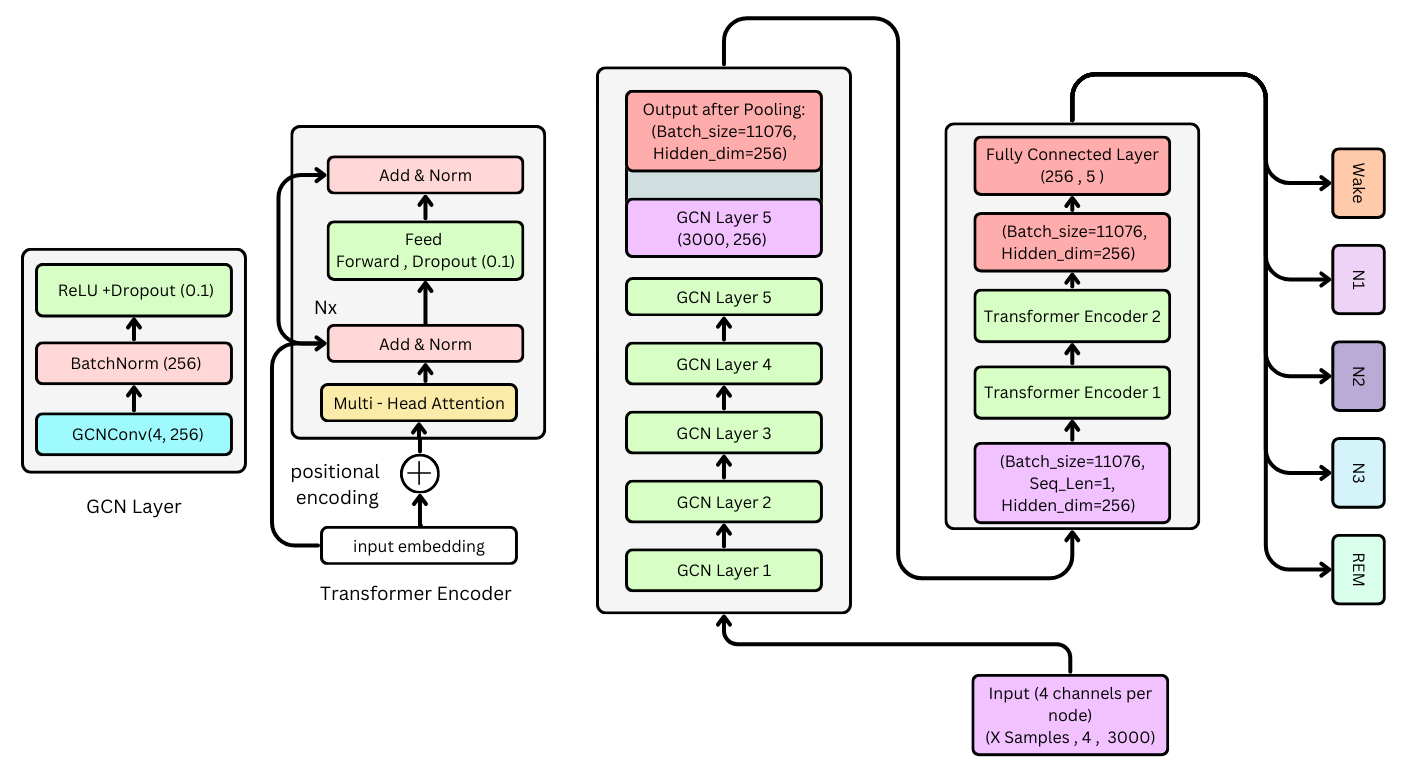
\includegraphics[width=1\linewidth]{img/Architechture.png}
    \caption{Proposed Architecture of GCN-Transformer Hybrid Approach}
    \label{fig:enter-label}
\end{figure}

\subsection{Input Data and Preprocessing}

We use EEG data represented as graph-structured inputs. Each sample contains 4 EEG channels recorded at 3000 frequency points. The dataset dimensions are:
\begin{itemize}
    \item \textbf{X\_all}: (11076, 4, 3000) - Samples, Channels, Frequency Points
    \item \textbf{Y\_all}: (11076,) - Labels for sleep stages
    \item Converted to PyTorch tensors:
    \begin{itemize}
        \item \textbf{X\_tensor}: torch.Size([11076, 4, 3000])
        \item \textbf{Y\_tensor}: torch.Size([11076])
    \end{itemize}
\end{itemize}

\subsubsection{Sleep Stage Mapping}

The sleep stages are mapped as follows:

\begin{table}[h]
\centering
\caption{Mapping of Original Sleep Stages to Labels}
\[
\begin{array}{|c|c|}
\hline
\textbf{Original Stage} & \textbf{Mapped Label} \\
\hline
\text{Sleep stage W} & 0 \\
\text{Sleep stage 1} & 1 \\
\text{Sleep stage 2} & 2 \\
\text{Sleep stage 3} & 3 \\
\text{Sleep stage 4} & 3 \\
\text{Sleep stage R} & 4 \\
\hline
\end{array}
\]
\label{tab:sleep_stage_mapping}
\end{table}


\subsubsection{Channel Selection}

The following EEG channels are selected for analysis: EEG Fpz-Cz, EEG Pz-Oz, EMG submental, and EOG horizontal.

\subsubsection{Preprocessing}

\textbf{Epoch Segmentation:}  
The EEG signals are segmented into 30-second epochs. Each epoch contains 3000 samples per channel, resulting in the final shape of the data as:

\[
\text{Final Data Shape: } [X, 4, 3000]
\]

\textbf{Band-Pass Filtering:}  
A band-pass filter with a frequency range of 0.3 - 30 Hz is applied to the signals. This removes frequencies outside this range, filtering out high-frequency noise and low-frequency drift.






\subsection{Graph Construction}

We represent each sample as a graph, where nodes correspond to EEG channels and edges represent spatial relationships. The graph is defined as:
\begin{itemize}
    \item \textbf{x}: Node features (shape: [3000, 4]) - EEG signals per channel
    \item \textbf{edge\_index}: Graph connectivity (shape: [2, 12])
    \item \textbf{y}: Sleep stage label for each sample (shape: [1])
\end{itemize}

\subsubsection{Methodology: Graph Dataset Creation}

The graph's adjacency matrix represents the spatial relationship between EEG channels. The edge weights are derived from the following graph adjacency matrix:

\begin{table}[h]
\centering
\caption{Graph Weight Representation}
\[
\begin{array}{|c|c|c|c|c|}
\hline
\textbf{} & \textbf{Fpz-Cz} & \textbf{Pz-Oz} & \textbf{EMG} & \textbf{EOG} \\
\hline
\textbf{Fpz-Cz} & 0 & 0.9 & 0.6 & 0.6 \\
\textbf{Pz-Oz}  & 0.9 & 0 & 0.6 & 0.6 \\
\textbf{EMG}    & 0.6 & 0.6 & 0 & 0.5 \\
\textbf{EOG}    & 0.6 & 0.6 & 0.5 & 0 \\
\hline
\end{array}
\]
\label{tab:correlation_matrix}
\end{table}


This matrix is used to define the weights of the edges between the EEG channels in the graph. The value at position \((i, j)\) indicates the weight of the edge between node \(i\) and node \(j\).

\begin{table}[ht]
\centering
\caption{Dataset shape Information}
\begin{tabular}{|c|c|}
\hline
\textbf{Component} & \textbf{Details} \\
\hline
\textbf{Total Samples} & 11,076 \\
\hline
\textbf{Example Sample Format} & Data(x=[3000, 4], edge index=[2, 12], edge attr=[12], y=[1]) \\
\hline
\textbf{x (Node features)} & EEG signals (shape: [3000, 4]) \\
\hline
\textbf{edge index} & Connectivity between EEG channels (shape: [2, 12]) \\
\hline
\textbf{edge attr} & Weights of edges between EEG channels (shape: [12]) \\
\hline
\textbf{y (Label)} & Sleep stage label for the sample (shape: [1]) \\
\hline
\end{tabular}

\end{table}


\subsubsection{Graph Representation of EEG Channels}
The EEG channels are represented as nodes in the graph, with edges indicating spatial relationships based on the adjacency matrix. The resulting graph structure captures both the spatial dependencies between the channels and the temporal dynamics of the EEG signals.
\begin{figure}[!h]
    \centering
    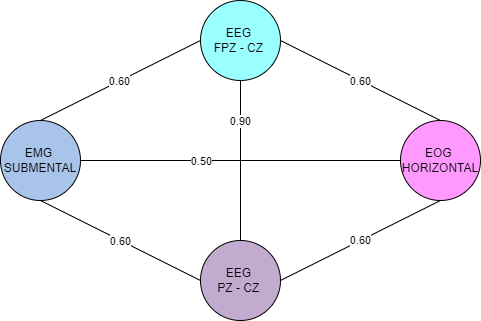
\includegraphics[width=0.5\linewidth]{img/Graph Weightage.png}
    \caption{Graph Weight Visulization}
    \label{fig:enter-label}
\end{figure}






\subsection{GCN Layers for Spatial Feature Extraction}

The GCN module captures spatial dependencies among EEG channels. We employ five Graph Convolutional Network (GCN) layers to learn the connectivity patterns between EEG channels, thereby enhancing feature extraction by leveraging the graph structure of EEG data. The architecture of each GCN layer is described as follows:

\begin{figure}
    \centering
    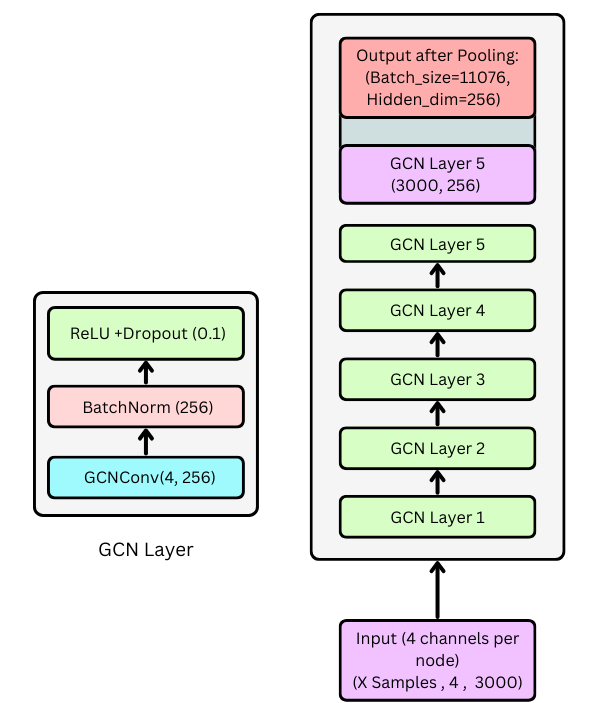
\includegraphics[width=0.7\linewidth]{img/Graph Convolution Neural Network.png}
    \caption{Graph Convolution Neural Network}
    \label{fig:enter-label}
\end{figure}
\begin{table}[ht]
\centering
\caption{GCN Layer Architecture}

\begin{tabular}{|c|c|}
\hline
\textbf{Layer} & \textbf{Operations} \\
\hline
\textbf{GCN Layer 1} & GCNConv(4, 256) $\rightarrow$ BatchNorm(256) $\rightarrow$ ReLU $\rightarrow$ Dropout(0.1) \\
\hline
\textbf{GCN Layer 2 to 5} & GCNConv(256, 256) $\rightarrow$ BatchNorm(256) $\rightarrow$ ReLU $\rightarrow$ Dropout(0.1) \\
\hline
\end{tabular}
\end{table}


 

 

The GCN layers work by taking the input features, which are of shape (4, 256) after the first layer, then passing them through a \textbf{Batch Normalization} layer with 256 output channels. The output is then activated using the \textbf{ReLU} activation function, formulated as:

\[
\text{ReLU}(x) = \max(0, x)
\]


This is followed by \textbf{Dropout}(0.1) for regularization, helping to avoid overfitting by randomly setting 10\% of the input units to zero.

After passing through all five GCN layers, the final output tensor has a shape of \( (3000, 256) \), representing 3000 frequency points with a 256-dimensional feature representation for each frequency point across all EEG channels.

To obtain a graph-level representation, we apply \textbf{global mean pooling} across nodes, which reduces the output to a \( \text{(Batch\_size}=11076, 256) \) tensor. This means that each sample is represented by a single 256-dimensional feature vector. The hidden dimension in this final layer is 256, which captures the most relevant features of the input data.



 

\subsection{Transformer Encoder for Temporal Dependencies}

\begin{table}[!h]
\centering
\caption{Transformer Encoder Overview}

\begin{tabular}{|c|c|}
\hline
\textbf{Component} & \textbf{Details} \\
\hline
\textbf{Preprocessing} & Expand graph embedding to (Batch\_size, 1, 256) \\
\hline
\textbf{Transformer Encoder} & 2 Transformer Encoder Layers \\
\hline
\textbf{d\_model (Hidden dimension)} & 256 \\
\hline
\textbf{nhead (Number of heads)} & 4 \\
\hline
\textbf{Dropout} & 0.1 \\
\hline
\textbf{batch first} & True \\
\hline
\textbf{Postprocessing} & Squeeze output to (Batch\_size, 256) \\
\hline
\textbf{Fully Connected Layer} & Linear(256 $\rightarrow$ 5) \\
\hline
\textbf{Output} & Logits for 5-class classification \\
\hline
\end{tabular}
\end{table}

\begin{figure}[!h]
    \centering
    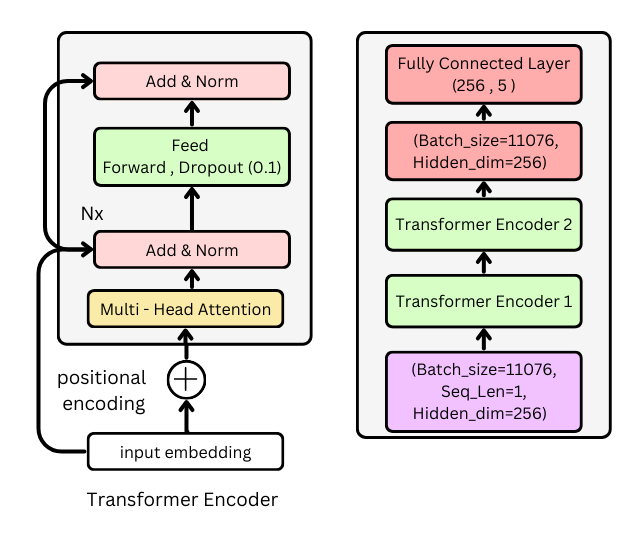
\includegraphics[width=0.7\linewidth]{img/transformer.png}
    \caption{Enter Caption}
    \label{fig:enter-label}
\end{figure}

The Transformer architecture follows the GCN layer pooling shapes. After pooling, the embeddings are passed through the multi-head attention mechanism, followed by Add \& Norm, which normalizes the output. This is then followed by a feed-forward layer, dropout with a 0.1 probability, and another Add \& Norm. The input embeddings are connected in parallel with the Add \& Norm. Positional encoding is applied during input to account for the temporal order of the sequence. The batch size is set to 1, with a sequence length of 1 and a hidden dimension of 256. The input passes through two Transformer Encoder layers, followed by a fully connected linear layer with a transformation from 256 to 5, which outputs the logits for 5-class classification. The final output is obtained using the softmax function, represented by:

\[
\text{Softmax}(z_i) = \frac{e^{z_i}}{\sum_j e^{z_j}}
\]



 
\subsection{Loss Function and Optimization}
We employ Focal Loss to address class imbalance, with parameters:
\begin{itemize}
    \item Gamma ($\gamma$): 3
    \item Label smoothing: 0.1
    \item Class weights computed from the dataset
\end{itemize}

The optimizer and learning rate scheduler are configured as follows:
\begin{itemize}
    \item \textbf{Optimizer}: AdamW (learning rate=0.0003, weight decay=1e-4)
    \item \textbf{Scheduler}: Cosine Annealing Learning Rate Scheduler
\end{itemize}

\subsubsection{Why Focal Loss Instead of Standard Cross-Entropy?}
\textbf{Motivation for Focal Loss:}  
Standard Cross-Entropy treats all samples equally, leading to bias towards majority classes. In imbalanced datasets, minority class predictions get suppressed. Focal Loss dynamically adjusts the loss contribution based on prediction confidence. It reduces the importance of well-classified samples and focuses more on hard-to-classify ones.

\textbf{Key Features of Focal Loss:}
\begin{itemize}
    \item Introduces a focusing parameter $\gamma$ to adjust class weighting.
    \item Includes class weighting factor $\alpha$ to handle imbalance.
    \item Works well for highly imbalanced datasets in classification tasks.
\end{itemize}

\subsubsection{Focal Loss Formulation}
The Focal Loss is formulated as follows:

\[
FL(p_t) = -\alpha (1 - p_t)^{\gamma} \log(p_t)
\]
where:
\begin{itemize}
    \item $p_t$ is the predicted probability for the target class.
    \item $\alpha$ is the weighting factor for class imbalance.
    \item $\gamma$ is the focusing parameter (higher values focus more on hard examples).
\end{itemize}

\subsubsection{Implementation Details}
\textbf{Label Smoothing:} Label smoothing is applied to prevent the log(0) issue by adding a small constant $\epsilon$:

\[
y_{\text{smooth}} = y(1 - \epsilon) + \frac{\epsilon}{C}
\]
where $C$ is the number of classes.

The PyTorch-based computation for Focal Loss with label smoothing becomes:

\[
L = \alpha (1 - p)^{\gamma} (-y_{\text{smooth}} \log p)
\]

\subsubsection{Why Use a Learning Rate Scheduler?}
\textbf{Importance of Learning Rate Scheduling:} The learning rate is crucial for training deep models efficiently. A high learning rate can lead to divergence, while a low one may cause slow convergence. Adaptive learning rate schedules help balance stability and speed.

\textbf{Why CosineAnnealingLR?} Cosine Annealing smoothly reduces the learning rate following a cosine decay. It starts with a large step size for exploration and gradually fine-tunes. This helps avoid sharp drops in the learning rate, improving generalization.

\subsubsection{Cosine Annealing Learning Rate Decay}
The learning rate decay is governed by the formula:

\[
\eta_t = \eta_{\min} + \frac{1}{2} (\eta_{\max} - \eta_{\min}) \left( 1 + \cos\left( \frac{T_{\text{cur}}}{T_{\text{max}}} \pi \right) \right)
\]
where:
\begin{itemize}
    \item $\eta_t$ is the learning rate at epoch $t$.
    \item $\eta_{\max}$ and $\eta_{\min}$ are the max/min learning rates.
    \item $T_{\text{cur}}$ is the current epoch.
    \item $T_{\text{max}}$ is the total number of epochs.
\end{itemize}

\textbf{Key Benefits:}
\begin{itemize}
    \item Encourages large updates early in training.
    \item Smoothly transitions into finer updates as training progresses.
    \item Helps the model avoid getting stuck in poor local minima.
\end{itemize}

\subsubsection{Training Methodology: Overview}
\textbf{SleepTrainer Class: Key Features:}
\begin{itemize}
    \item Handles model training, validation, and optimization.
    \item Uses Focal Loss to address class imbalance.
    \item Applies CosineAnnealingLR scheduler for smooth learning rate decay.
\end{itemize}

\textbf{Training Process:}
\begin{itemize}
    \item Compute class weights for imbalanced data.
    \item Iterate through training batches, compute loss, and update weights.
    \item Validate model performance on a separate validation set.
    \item Adjust learning rate dynamically using a scheduler.
\end{itemize}

\subsubsection{Training Methodology: Hyperparameters}
\textbf{Key Hyperparameters:}
\begin{itemize}
    \item Batch Size: 32
    \item Learning Rate: 0.0003
    \item Weight Decay: 1e-4
    \item Epochs: 20
    \item Optimizer: AdamW
    \item Learning Rate Scheduler: CosineAnnealingLR
\end{itemize}
Gradually reduces learning rate over time for smooth convergence, helping prevent sudden drops in performance.

\subsubsection{Training Methodology: Handling Class Imbalance}
\textbf{Why Compute Class Weights?}  
EEG sleep data is imbalanced, with some sleep stages appearing more frequently. Without weighting, the model may favor majority classes. Weights ensure rare classes contribute more to the loss.

\textbf{Class Weight Computation:}
The class weight for class $c$ is computed as:

\[
w_c = \left( \frac{\text{Total Samples}}{\text{Class Count} + 1} \right)^{0.5}
\]
where:
\begin{itemize}
    \item $w_c$ is the computed weight for class $c$.
    \item Smaller classes receive higher weights.
\end{itemize}

These weights are applied to the Focal Loss during training.






 
